% !TeX encoding = UTF-8
% !Tex spellcheck = de_DE

\documentclass[10pt,a4paper]{article}
% ***********************************************************
% ***************** MyStyle - Rene Vollmer*******************
% ***********************************************************
% Version 1.0b



\usepackage[utf8]{inputenc}

\usepackage{hyperref}

\usepackage{amsmath} % AMS Math Package
\usepackage{amsfonts}
\usepackage{amsthm} % Theorem Formatting
\usepackage{amssymb}	% Math symbols such as \mathbb
\usepackage{mathtools}
\usepackage{graphicx} % Allows for eps images
\usepackage{multicol} % Allows for multiple columns
\usepackage[]{units}

\usepackage{hyperref} %Links
\usepackage{url}

\usepackage{verbatim} %Fuer mehrzeilige kommentare \begin{comment} \end{comment}

\usepackage[hang]{caption} % Captions einrücken
\usepackage{subfigure}

%Some other shit
\usepackage{float}
%\floatstyle{boxed} %Puts a box around each figure
\restylefloat{figure}
%\usepackage{wrapfig}
\usepackage{microtype}



\usepackage{xparse} % For uses like \DeclareDocumentCommand{\foocmd}{ O{default1} O{default2} m }{#1~#2~#3}


%\usepackage{color}
%\definecolor{gray}{rgb}{.5,.5,.5}
%\definecolor{lightgray}{rgb}{.25,.25,.25}

%Graphics (PGF / TIKZ) **+**+**+**+**+**+**+**+**+**+**+**+**+**+
\usepackage{tikz}
\usetikzlibrary{patterns}
\tikzset{
	hatchhor/.style={pattern=horizontal lines,pattern color=#1},
	hatchhor/.default=black
}
\tikzset{
	hatchvert/.style={pattern=vertical lines,pattern color=#1},
	hatchvert/.default=black
}
\tikzset{
	hatchdiag/.style={pattern=north east lines,pattern color=#1},
	hatchdiag/.default=black
}
\tikzset{
	hatchdiag2/.style={pattern=north west lines,pattern color=#1},
	hatchdiag2/.default=black
}
%also possible grid, crosshatch, dots, crosshatch dots, fivepointed stars, sixpointed stars

\usepackage{pgfplots}
\usepgfplotslibrary{fillbetween}

% Style to select only points from #1 to #2 (inclusive)
\pgfplotsset{select coords between index/.style 2 args={
		x filter/.code={
			\ifnum\coordindex<#1\def\pgfmathresult{}\fi
			\ifnum\coordindex>#2\def\pgfmathresult{}\fi
		}
	}
}


\newcommand{\vasymptote}[2][]{
	\draw [color=gray,densely dashed,#1] ({rel axis cs:0,0} -| {axis cs:#2,0}) -- ({rel axis cs:0,1} -| {axis cs:#2,0});
}

\newcommand{\vertline}[2][]{
	\draw [#1] ({rel axis cs:0,0} -| {axis cs:#2,0}) -- ({rel axis cs:0,1} -| {axis cs:#2,0});
}
%END Graphics **+**+**+**+**+**+**+**+**+**+**+**+**+**+**+**+**+

%Stolen from http://www.dfcd.net/articles/latex/latex.html
% **#**#**#**#**#**#**#**#**#**#**#**#**#**#**#**#**#**#**#**#**#
\makeatletter % Need for anything that contains an @ command

\let\vaccent=\v % rename builtin command \v{} to \vaccent{}
\renewcommand{\v}[1]{\ensuremath{\mathbf{#1}}} % for vectors
\newcommand{\gv}[1]{\ensuremath{\mbox{\boldmath$ #1 $}}} 
% for vectors of Greek letters
\newcommand{\uv}[1]{\ensuremath{\mathbf{\hat{#1}}}} % for unit vector
\newcommand{\abs}[1]{\left| #1 \right|} % for absolute value
\newcommand{\avg}[1]{\left< #1 \right>} % for average
\let\underdot=\d % rename builtin command \d{} to \underdot{}
\renewcommand{\d}[2]{\frac{d #1}{d #2}} % for derivatives
\newcommand{\niced}[2]{\nicefrac{d #1}{d #2}} % for in-text-derivatives
\newcommand{\nicedd}[2]{\nicefrac{d^2 #1}{d #2^2}} % for double derivatives\newcommand{\dd}[2]{\frac{d^2 #1}{d #2^2}} % for in-text-double derivatives
\newcommand{\pd}[2]{\frac{\partial #1}{\partial #2}} 
% for partial derivatives
\newcommand{\pdd}[2]{\frac{\partial^2 #1}{\partial #2^2}} 
% for double partial derivatives
\newcommand{\pdc}[3]{\left( \frac{\partial #1}{\partial #2}
	\right)_{#3}} % for thermodynamic partial derivatives
\newcommand{\ket}[1]{\left| #1 \right>} % for Dirac bras
\newcommand{\bra}[1]{\left< #1 \right|} % for Dirac kets
\newcommand{\braket}[2]{\left< #1 \vphantom{#2} \right|
	\left. #2 \vphantom{#1} \right>} % for Dirac brackets
\newcommand{\matrixel}[3]{\left< #1 \vphantom{#2#3} \right|
	#2 \left| #3 \vphantom{#1#2} \right>} % for Dirac matrix elements
\newcommand{\grad}[1]{\gv{\nabla} #1} % for gradient
\let\divsymb=\div % rename builtin command \div to \divsymb
\renewcommand{\div}[1]{\gv{\nabla} \cdot #1} % for divergence
\newcommand{\curl}[1]{\gv{\nabla} \times #1} % for curl
\let\baraccent=\= % rename builtin command \= to \baraccent
\renewcommand{\=}[1]{\stackrel{#1}{=}} % for putting numbers above =
\newtheorem{prop}{Proposition}
\newtheorem{thm}{Theorem}[section]
\newtheorem{lem}[thm]{Lemma}
\theoremstyle{definition}
\newtheorem{dfn}{Definition}
\theoremstyle{remark}
\newtheorem*{rmk}{Remark}
% **#**#**#**#**#**#**#**#**#**#**#**#**#**#**#**#**#**#**#**#**#


%Equalssign with hat/corresponds to   \equalhat
\newcommand\equalhat{%
	\stackrel{\Lambda}{=}
}
%Equalssign with !
\newcommand\shallbe{%
	\stackrel{!}{=}
}
% := and =:
\newcommand{\defeq}{\vcentcolon=}
\newcommand{\eqdef}{=\vcentcolon}



%Encirecled Numbers, used in Graphics
\let\depth\relax
\def\X#1{%
	%#1%
	%\textcircled{#1}%
	\raisebox{0.9pt}{\textcircled{\raisebox{-.9pt}{#1}}}%
	%\ding{\numexpr171+#1\relax}%
}


% ******************************~~~~*****************************
%Photo quality management. This is an old try:
\newcommand\openfile{\newwrite\outputstream\immediate\openout\outputstream=photo.log
	\writetofile[linewidth]{\the\linewidth}
	\writetofile[textwidth]{\the\textwidth}
	\writetofile[dpi]{300}
	}
\newcommand\closefile{\immediate\closeout\outputstream}
\newcommand\writetofile[2][2]{\immediate\write\outputstream{#1 #2}}

\newcommand\photo[2][2]{\includegraphics[width=#1]{#2}\writetofile[#2]{#1}}

% ***************************************************************
% And this is working
% Reduce image size for fixed dpi
% Introduce \includegraphicsRS for this purpose

% for downsampling large images: \includegraphicsRS
% (\includegraphics "resize")
% \includegraphicsRS[#1][#2]{#3}
% #1 = normal \includegraphics[] - Parameter (like scale=1) {optional}
% #2 = approx part of the screen, eg half page width use 0.5 or 1/2 {optional}
%      reduces to #2*1000px
% #3 = relative path to image file WITH ending (e.g. .jpg) {required}
\pdfimageresolution 300

\newcommand{\includegraphicsRS}{}

\ifnum\pdfshellescape=1
% Yes, enabled
% IFP - image file path
% IFN - image filename only
% here resizing at #2*1000 px wide
\newread\myinput
% must add default argument [] so typeout works
\DeclareDocumentCommand{\includegraphicsRS}{ O{\@empty} O{1} m }{ %
%\renewcommand\includegraphicsRS[2][\@empty]{
	% run downsampling bash script
	\immediate\write18{mkdir -p images; mkdir -p images/downsampled; IFP=#3 ; %
		PIX=#2 ; PIX=$( awk  'BEGIN { rounded = sprintf("\%.0f", ('$PIX')*1000); print rounded }' ) ;
		echo "$PIX 1000 *p" | dc ; %
		echo "Processing $IFP" ; %
		IFN=$(basename $IFP) ; %
		echo "images/downsampled/$IFN" > tmpname ; %
		if [ ! -f images/downsampled/$IFN ]; then %
		echo "File images/downsampled/$IFN not found! Converting..." ; %
		%the \string> after the pixel width (e.g. 1000x) will prevent imagemagick from producing files larger than the original
		convert $IFP -resize $PIX"x\string>" -quality 85 images/downsampled/$IFN ; %

		else %
		echo "Found images/downsampled/$IFN - reusing." ; %
		fi ; %
		%alternatively: bash includegraphicsRS.sh #3 #2
		%and have the code in the *.sh-file.
	} % end write18
	% here we should have downsampled file
	% retrieve downsample filename first
	\immediate\openin\myinput=tmpname
	% The group localizes the change to \endlinechar
	\bgroup
	\endlinechar=-1
	\immediate\read\myinput to \localline
	% Since everything in the group is local, we have to explicitly make the
	% assignment global
	\global\let\myTmpFileName\localline
	\egroup
	\immediate\closein\myinput
	% Clean up after ourselves
	% \immediate\write18{rm -f -- tmpname}
	% finally, include downsampled image
	\includegraphics[#1]{\myTmpFileName}
} % end renewcommand
\else
% No, disabled
% in this case, \includegraphicsRS is just the usual \includegraphics
\renewcommand\includegraphicsRS[2][\@empty]{%
	\includegraphics[#1]{#2}
}
\fi

\begin{comment}
old stuff, not used any longer. Could be useful for future changes though.
\usepackage{fp}

\newlength{\TOarg} \newlength{\TOunit}
{\catcode`p=12 \catcode`t=12 \gdef\TOnum#1pt{#1}}
\newcommand\TOop[2]{\setlength{\TOarg}{#2}%
	\FPdiv\TOres{\expandafter\TOnum\the\TOarg}{\expandafter\TOnum\the\TOunit}%
	\FPround\TOres\TOres{#1}}
\newcommand{\TOspace}{\ }
\newcommand\TOpt[2][2]{\setlength{\TOunit}{1pt}\TOop{#1}{#2}\TOres\TOspace pt}
\newcommand\TOin[2][2]{\setlength{\TOunit}{1in}\TOop{#1}{#2}\TOres\TOspace in}
\newcommand\TOcm[2][2]{\setlength{\TOunit}{1cm}\TOop{#1}{#2}\TOres\TOspace cm}
\newcommand\TOmm[2][2]{\setlength{\TOunit}{1mm}\TOop{#1}{#2}\TOres\TOspace mm}
\newcommand\TOem[2][2]{\setlength{\TOunit}{1em}\TOop{#1}{#2}\TOres\TOspace em}
\newcommand\TOpx[2][2]{\setlength{\TOunit}{1px}\TOop{#1}{#2}\TOres\TOspace px}
\newcommand\TOptdeux[2][2]{\setlength{\TOunit}{1pt}\TOop{#1}{#2}\TOres}

convert $IFP -resize 50\% images/downsampled/$IFN ; %		textwidth="\the\textwidth" ; %
TW=${textwidth:0:(-2)} ; %
VARI="$TW"; %
convert -resize 2000x -units pixelspercentimeter $IFP -density 120 -pointsize 30 -draw "gravity south-east fill black text 0,5 '$VARI'" downsampled/$IFN ; %
\end{comment}


% END of \includegraphicsRS
% ***************************************************************
% ******************************~~~~*****************************



% ***********************************************************
% ********************** END HEADER *************************
% ***********************************************************


% Literaturangabe
%\usepackage{biblatex}
%\bibliographystyle{plain}
\bibliographystyle{alpha} %http://sites.stat.psu.edu/~surajit/present/bib.htm
%\usepackage{natbib}
%\bibliographystyle{plainnat}


\begin{comment}
\usepackage{titlesec}
\titleformat{\subsection}[runin]% runin puts it in the same paragraph
{\normalfont\bfseries}% formatting commands to apply to the whole heading
{\thesubsection}% the label and number
{0.5em}% space between label/number and subsection title
{}% formatting commands applied just to subsection title
[]% e.g. [.] punctuation or other commands following subsection title\frac{•}{•}
\end{comment}


\linespread{1.1}
\usepackage{microtype}

%\addto\captionsgerman{ \renewcommand{\figurename}{\small{\textbf{Abb.}}}
%\captionsetup{figurewithin = section}
%\captionsetup{font=small, labelfont=bf} }


\begin{document}
	
	\pagenumbering{Roman}
	%TODO REMOVE
	\textbf{TODO}
	
René
\begin{enumerate}
	\item Regina sagen, dass sie auf die Eigenschaften der FT refen soll
	\item Regine Videos vom Handy geben
	\item Regina Rücktransformierte Bilder geben
	\item 
\end{enumerate}

Vivi
\begin{enumerate}
	\item @ rené: ich hab bei der section "einkopplung" jetzt keine unsrer Leistungs-berechnungs- rechnungen hingeschrieben, weil die ja alle für die photodiode waren, mit irgendwelchen zu großen widerständen... 
	\item ...
\end{enumerate}
	
	
	%Metadaten
	\title{\textit{Fortgeschrittenenpraktikum}\\-\\Optische Fouriertransformation }
	\date{23.02.2015}
	\author{Vivien Sleziona \footnote{vivi.s@arcor.de}\\ Regina Schauer \footnote{regina.schauer@web.de}\\ René Vollmer \footnote{rene.vollmer@studium.uni-hamburg.de} \\ \\Betreut durch\\ Kai Morgener\footnote{kmorgene@physnet.uni-hamburg.de}}
	
	\maketitle
	
	\begin{center} 
		\bigskip
		\bigskip
		
		\begin{minipage}{0.75\textwidth}
			% !TeX root = ../praktikum.tex
% !TeX encoding = UTF-8
% !Tex spellcheck = de_DE

Die Fourier-Analytik und insbesondere die Fouriertransformation sind auf vielen modernen Anwendungen kaum noch weg zu denken. Sie ist essentieller Bestandteil vieler Bildverarbeitungsalgorithmen\cite{easton_fourier_2010} und -kompressionsverfahren wie JPEG\cite{_jpeg_2015}, sie wird genutzt um Bildinformationen Computeralgorithmen zugänglich zu machen\cite{prof._dr._norbert_link_vorlesungsscript:_????} und in vielen anderen Bereichen der Signalverarbeitung.\\

In diesem Versuch soll mit einfachen optischen Mitteln eine Fouriertransformation auf Bildern durchgeführt, die Fouriertransformierte manipuliert und rücktransformiert werden. Dabei wird dem Leser ein intuitives Verständnis für die Funktionsweise und Bedeutung von Fouriertransformationen vermittelt werden.
		\end{minipage}
	\end{center}
	
	%\vfill
	\newpage
	
	\tableofcontents
	\vfill
	\newpage
	\clearpage	
	
	\pagenumbering{arabic}
	
	\section{Theoretical Concepts}
	
	% !TeX root = ../praktikum.tex
% !TeX encoding = UTF-8
% !Tex spellcheck = de_DE

\begin{align}
	\vec{\j} = \mathbf{\sigma} \cdot \vec{E} & & \Leftrightarrow & & \vec{E} = \mathbf{\rho} \cdot \vec{j}
	\label{eq:u2rho}
\end{align}

	
	\newpage
	\clearpage
	
	\section{Experimental Procedure} %Setup and conduct of the experiment
	\subsection{Einkopplung}
	% !TeX root = ../praktikum.tex
% !TeX encoding = UTF-8
% !Tex spellcheck = de_DE

	\subsection{Lichtsensor}
	% !TeX root = ../praktikum.tex
% !TeX encoding = UTF-8
% !Tex spellcheck = de_DE

Für die Optimierung der Einkopplungsleistung wurde ein Powermeter benutzt. Dieses wurde an ein digitales Oszilloskop angeschlossen, um schnelle Änderungen zu visualisieren und so den Optimierungsvorgang, insbesondere das \textit{Walken}, zu erleichtern. Da diese Powermeter mit recht hohen Anschaffungskosten einher gehen, wurde in diesem Versuchsteil versucht, eine Leistungsmessung des Laserlichtes mit einer Photodiode zu messen.\\

Die verwendete Photodiode\footnote{Modell OSD15-5T von CENTRONIC\cite{farnell.com_osd15-5t_????}} produziert laut Datenblatt einen Strom von \unit[0,18-0,21]{mA} pro Milliwatt eingestrahlter Lichtleistung bei \unit[436]{nm} Wellenlänge. Da Strom nicht direkt gemessen werden kann, wird ein Widerstand parallel geschaltet und der Spannungsabfall über diesen nach $U=R\cdot I$ mit einem Oszilloskop gemessen. Wenn man für \unit[1]{mW} Lichtleistung einen Spannungsabfall von \unit[100]{mV} erreichen möchte, würde man einen $\nicefrac{U}{I}=\nicefrac{\unit[100]{mV}}{\unit[0,2]{mA}}=\unit[500]{\Omega}$ Widerstand verwenden. Da dies jedoch ein sehr kleiner Messbereich ist, wurden \unit[4]{V} pro Milliwatt angesetzt und entsprechend ein \unit[20]{$k\Omega$} Widerstand verwendet.\\

Bei sehr schwachen Lichteinfall (Deckenlampe, Fenster aus der Ferne, ...) konnte auf dem Oszilloskop eine Schwankung in der Spannung festgestellt werden. Bei hohen Lichtleistungen fallen diese Schwankungen sehr klein aus. Für andere Widerstandswerte, z.B. 10 oder \unit[100]{$k\Omega$}, erhält man nahezu identische Werte um \unit[440]{mV}. Da dies in etwa der Bandlücke eines PN-Überganges entspricht, liegt die Vermutung nahe, dass dies eine Sättigungserscheinung ist.

Daher wurde der Aufbau mit kleineren Widerstandswerten von 500 und \unit[1000]{$\Omega$} getestet. Die gemessenen Spannungen sowie die dazu vom Powermeter abgelesenen Werte für die Lichtleistung sind in Abbildung~\ref{fig:photodiode} aufgetragen.


\begin{figure}[ht]
	\centering
	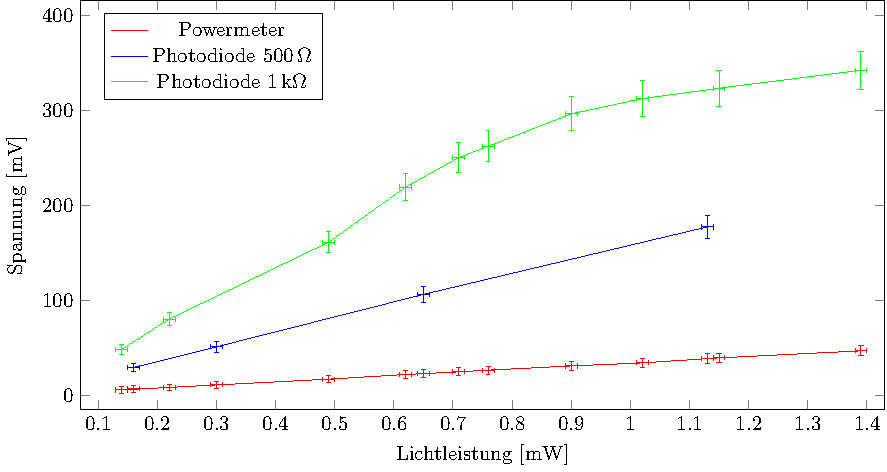
\includegraphics[width=1\linewidth]{graphs/fotodiode/diode.pdf}
	\caption[Vermessung einer Photodiode]{
		Spannungen gemessen über je einen zu einer Photodiode parallel geschalteten Widerstand mit 500 und \unit[1000]{$\Omega$}. Zusätzlich ist der Verlauf der Spannung eines Powermeters aufgetragen.
	}
	\label{fig:photodiode}
\end{figure}

Es ist für \unit[1]{$k\Omega$} eine Sättigung ab etwa \unit[0,9]{mW} erkennbar, die Variante mit \unit[500]{$\Omega$} weist im gesamten Messbereich ein sehr lineares Verhalten auf. Die Fehlerbalken in der x-Achse wurden zu \unit[0,01]{mW} gewählt, da das Powermeter nur zwei Nachkommastellen anzeigt. Der Fehler in der y-Achse wurde auf etwa 5\% gewählt.

%Bei dieser Wellenlänge hat die Photodiode eine Effizienz von etwa \unit[20]{\%} bei der Umwandlung von Licht zu Strom. Bei \unit[660]{nm} (Frequenz des Lasers) etwa \unit[40]{\%}.

	\subsection{Abbildung und Fourierbild}
	% !TeX root = ../praktikum.tex
% !TeX encoding = UTF-8
% !Tex spellcheck = de_DE


Im letzten Versuchsteil wurde der Laserstrahl am anderen Ende der Glasfaser ausgekoppelt und auf einen optischen Pfad gesandt, um Abbildungen von Objekten und deren Fourierspektren, sowie die Veränderung der Abbildung bei Maniplation des Fourierspektrums zu beobachten. Hierfür wurde hinter dem Faserauskoppler der Aufbau aus Abbildung \ref{fig:4f-aufbau} realisiert.

\begin{figure}[h]
	\centering
	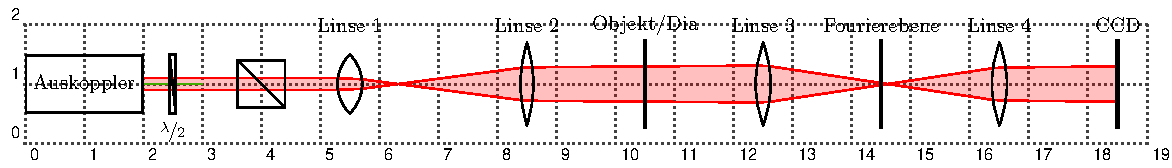
\includegraphics[width=1\linewidth]{graphs/versuchsaufbau/4f-aufbau.pdf}
	\caption[Schematische Skizze des 4f-Aufbaus]{
		Schematische Skizze des 4f-Aufbaus. Der Laserstrahl passiert nach Verlassen des Auskopplers eine $\nicefrac{\lambda}{2}$-Platte und anschließend einen Strahlteiler. Der zweite Teil des Strahls, welcher vom Strahlteiler abgelenkt wird, trifft auf eine Strahlblockierung und wird nicht weiter verwendet. Zwischen Linse 2 und 3 befindet sich die Halterung für das Objekt/Dia, in der Fourierebene wird entweder eine zweite Kamera oder ein Filter positioniert. Die CCD Kamera am Ende des Strahlengangs befindet sich in der Abbildungsebene des Aufbaus.
	}
	\label{fig:4f-aufbau}
\end{figure}

In diesem, sogenannten 4f-Aufbau, passierte der Laserstrahl nach der Reflektion am ersten Spiegel eine $\nicefrac{\lambda}{2}$-Platte und dahinter einen Strahlteiler. Mithilfe des Strahlteilers wurde eine eindeutige Polarisierung sicher gestellt, während mit dem Plättchen die Lichtmenge der durchlässigen Polarisation eingestellt werden konnte.\\

Um die abzubildenden Objekte vollständig ausleuchten zu können, wurde der Laserstrahl in diesem Aufbau mit Hilfe der ersten beiden Linsen aufgeweitet und wieder kollimiert. Im Brennpunkt der dritten Linse befand sich ein Objektträger in der Gegenstandsebene. In diesem wurden die abzubildenden Objekte angebracht. Die Fourierebene befindet sich im Brennpunkt der Linsen 3 und 4. Nach der vierten Linse wird der Strahl erneut kollimiert und trifft auf die CCD Kamera, Kamera 1. Hier wird das Objekt möglichst originalgetreu abgebildet. Um Aufnahmen der Fourierspektren zu erhalten, wurde bei Bedarf eine zweite Kamera, Kamera 2, in der Fourierebene montiert. \\ 

Verwendet wurden hierbei Linsen der Brennweiten wie folgt: Linse 1 mit $f_{1}=\unit[20]{mm}$, Linse 2 mit $f_{2}=\unit[200]{mm}$, Linse 3 und 4 mit $f_{3}=f_{4}=\unit[100]{mm}$. Direkt hinter der Auskopplung wurde zusätzlich ein Spiegel, optimiert für Wellenlängen zwischen \unit[400-700]{nm}, in den 4f-Aufbau aufgenommen, um den Verlauf des Laserstrahls im optischen Pfad besser feinjustieren zu können. Leider wurde die Strahlqualität durch diesen stark beeinträchtigt, so dass zusätzlich ein Pinhole zwischen Linse 1 und 2 notwendig war, um eine gaußähnliche Strahlmode zu erhalten.\\


\begin{figure}[h]
	\centering
	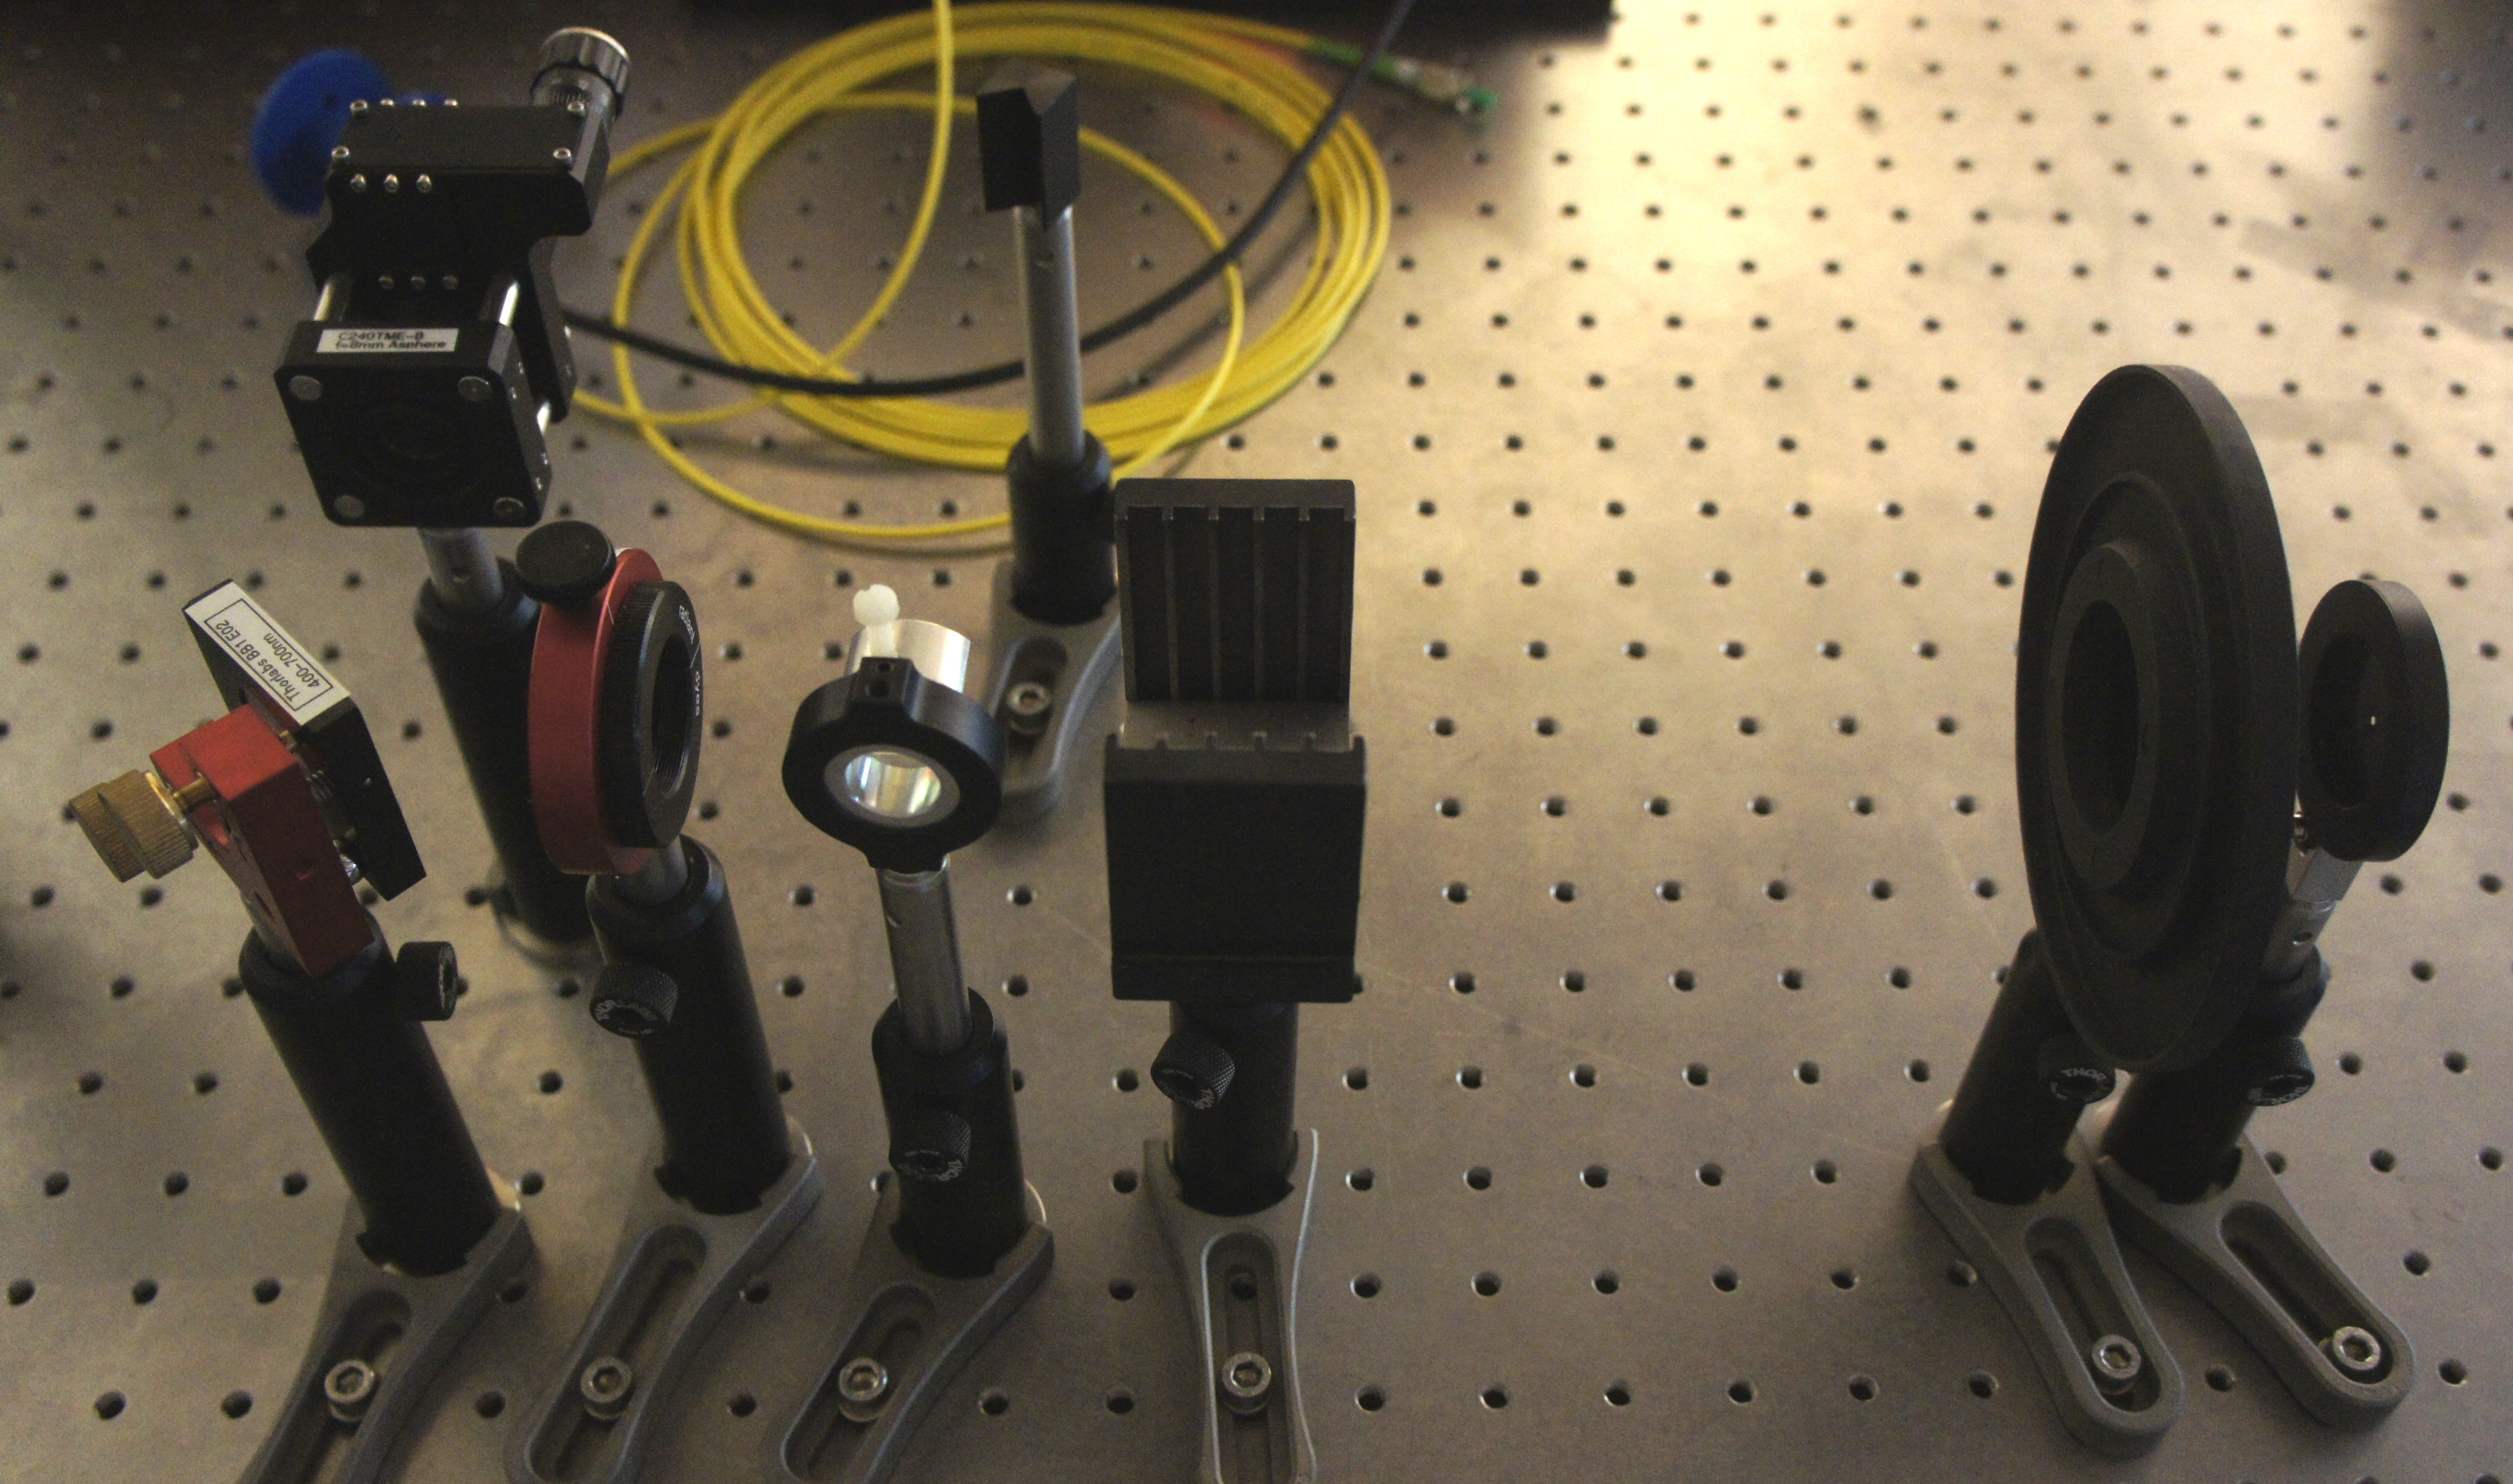
\includegraphics[width=0.7\linewidth]{images/4f-anfang.JPG}
	\caption[Vorderer Teil des 4f-Aufbaus]{
		Vorderer Teil des realisierten 4f-Aufbaus. Am rechten Bildrand ist das Pinhole hinter Linse 1 zu sehen.
	}
	\label{fig:_DSC7961}
\end{figure}

\begin{figure}[ht]
	\centering
	\includegraphicsRS[width=0.43\linewidth]{images/_DSC7988.JPG}~
	\includegraphicsRS[width=0.43\linewidth]{images/IMG_2223.jpg}
	%\vspace{2cm}\hspace{2cm}
	\caption{
		\textbf{Links:} Mode des Laserstrahls am Ende des optischen Pfades vor Einbau des Pinholes.\\
		\textbf{Rechts:} Mode des Laserstrahls am Ende des optischen Pfades nach Einbau des Pinholes.
	}
	\label{fig:_DSC7988}
\end{figure}

%TODO: Ein bisschen was über die Justierung erzählen

Als Hilfsmittel bei der Justage 




\begin{comment}
\begin{figure}
	\centering
	\includegraphicsRS[width=0.7\linewidth, angle=90]{images/_DSC7967.JPG}
	\caption{Foto des hier realisierten 4f-Aufbaus.}
	\label{fig:_DSC7967}
\end{figure}
\end{comment}

\clearpage


Nachdem der 4f-Aufbau montiert und der Verlauf des Laserstrahls im optischen Pfad optimiert war, wurden nacheinander die Objekte 1 bis 5 (siehe Abbildung~\ref{fig:Objekte-aus-Anleitungsheft}) in Form von Dias in dem Objektträger montiert.

%TODO: GgF diese Bilder je mit in die Reihe der Abbildung 9-21 Bilder machen.
\begin{figure}[h]
	\centering
	\includegraphicsRS[width=0.15\textwidth]{images/Anleitungsheft/objekt1.png}~~
	\includegraphicsRS[width=0.15\textwidth]{images/Anleitungsheft/objekt2.png}~~
	\includegraphicsRS[width=0.15\textwidth]{images/Anleitungsheft/objekt3.png}~~
	\includegraphicsRS[width=0.15\textwidth]{images/Anleitungsheft/objekt4.png}~~
	\includegraphicsRS[width=0.15\textwidth]{images/Anleitungsheft/objekt5.png}
	\caption[Die zur Messung verwendeten Diamotive]{
		Darstellung der zur Messung verwendeten Diamotive. Im Text werden diese Objekt mit Objekt 1 bis 5, von links nach rechts, bezeichnet..
	}
	\label{fig:Objekte-aus-Anleitungsheft}
\end{figure}

Anhand der Dias wurden zunächst sowohl Kamera 1, als auch Kamera 2 nachjustiert, bis ein möglichst scharfes Bild auf dem über das Programm \textit{uc480 Viewer-DCC1545M-ID} angeschlossenen Bildschirm zu erkennen war. Mit den beiden Kameras wurden nacheinander für jedes der Objekte Aufnahmen in der Abbildungsebene und zugehörig zu jeder Einstellung auch in der Fourierebene gemacht (Siehe Abbildungen~\ref{fig:example1}-\ref{fig:example16}).

\begin{figure}[h]
	\centering
	%\includegraphicsRS[width=0.7\linewidth]{images/example1.png}
	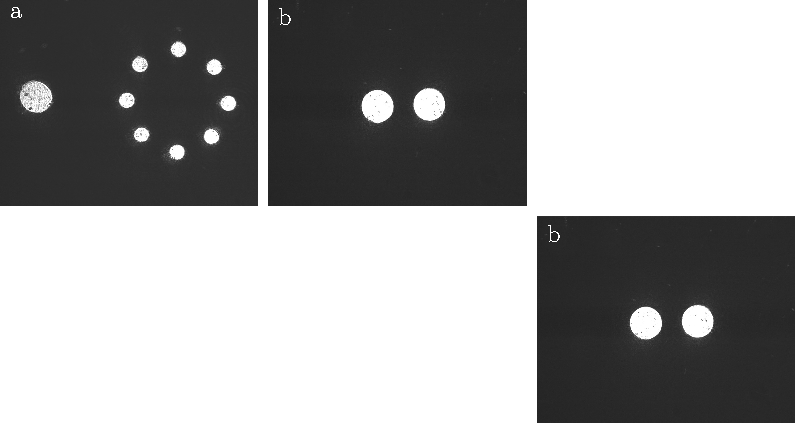
\includegraphics{images/ergebniss_ex1/abb.pdf}
	\caption{
		Beispiel von Abbildung (links) und Fourierspektrum (rechts) für Objekt 1.
	}
	\label{fig:example1}
\end{figure}

\begin{figure}[h]
	\centering
	\includegraphicsRS[width=0.7\linewidth]{images/example2.png}
	\caption{Beispiel von Abbildung (links) und Fourierspektrum (rechts) für Objekt 2}
	\label{fig:example2}
\end{figure}

\begin{figure}[h]
	\centering
	\includegraphicsRS[width=0.7\linewidth]{images/example3.png}
	\caption{Beispiel einer anderen Abbildung (links) und entsprechendes Fourierspektrum (rechts) für Objekt 2}
	\label{fig:example3}
\end{figure}

\begin{figure}[h]
	\centering
	\includegraphicsRS[width=0.7\linewidth]{images/example13.png}
	\caption{Beispiel von Abbildung (links) und Fourierspektrum (rechts) für Objekt 3}
	\label{fig:example13}
\end{figure}

\begin{figure}[h]
	\centering
	\includegraphicsRS[width=0.7\linewidth]{images/example4.png}
	\caption{Beispiel von Abbildung (links) und Fourierspektrum (rechts) für Objekt 4}
	\label{fig:example4}
\end{figure}

\begin{figure}[h]
	\centering
	\includegraphicsRS[width=0.7\linewidth]{images/example9.png}
	\caption{Beispiel einer weiteren Abbildung (links) und entsprechendes Fourierspektrum (rechts) für Objekt 4}
	\label{fig:example9}
\end{figure}

\begin{figure}[h]
	\centering
	\includegraphicsRS[width=0.7\linewidth]{images/example16.png}
	\caption{Beispiel von Abbildung (links) und Fourierspektrum (rechts) für Objekt 5}
	\label{fig:example16}
\end{figure}


\clearpage\newpage %TODO: Remove
Wie die Abbildungen \ref{fig:example1} bis \ref{fig:example16} zeigen, konnte hier beobachtet werden, dass die aus der Theorie zu erwartenden Fourierspektren mit Kamera 2 in der Fourierebene tatsächlich sichtbar gemacht werden konnten. 
Zudem wurden für die Objekte 4 und 5 verschiedene Filter in die Fourierebene gestellt und Aufnahmen der Kamera 1 in der Abbildungsebene gemacht. Für Objekt 4 wurde hierzu ein Tiefpass und mehrere Breitbandfilter verwendet. Für Objekt 5 wurde ein Halbebenenfilter horizontal, vertikal und diagonal in die Fourierebene gehalten. \\


\begin{figure}[h]
	\centering
	\includegraphicsRS[width=0.7\linewidth]{images/example10_Filter1B.png}
	\caption{
		\textbf{Links:} Beispielaufnahme von Objekt 4 aus der Abbildungsebene.\\
		\textbf{Rechts:} Aufnahme des gleichen Objekts aus der Abbildungsebene mit Filter 1B in der Fourierebene}
	\label{fig:example10_Filter1B}
\end{figure}

\begin{figure}[h]
	\centering
	\includegraphicsRS[width=0.7\linewidth]{images/example11_Filter1C.png}
	\caption{
		\textbf{Links:} Beispielaufnahme von Objekt 4 aus der Abbildungsebene.\\
		\textbf{Rechts:} Aufnahme des gleichen Objekts aus der Abbildungsebene mit Filter 1C in der Fourierebene
	}
	\label{fig:example11_Filter1C}
\end{figure}

\begin{figure}[h]
	\centering
	\includegraphicsRS[width=0.7\linewidth]{images/example12_Filter1D.png}
	\caption{links: Beispielaufnahme von Objekt 4 aus der Abbildungsebene. Rechts: Aufnahme des gleichen Objekts aus der Abbildungsebene mit Filter 1D in der Fourierebene}
	\label{fig:example12_Filter1D}
\end{figure}

\begin{figure}[h]
	\centering
	\includegraphicsRS[width=0.7\linewidth]{images/example17.png}
	\caption{links: Beispielaufnahme von Objekt 4 aus der Abbildungsebene. Rechts: Aufnahme des gleichen Objekts aus der Abbildungsebene mit vertikalem Halbebenenfilter in der Fourierebene}
	\label{fig:example17}
\end{figure}

\begin{figure}[h]
	\centering
	\includegraphicsRS[width=0.7\linewidth]{images/example18.png}
	\caption{links: Beispielaufnahme von Objekt 4 aus der Abbildungsebene. Rechts: Aufnahme des gleichen Objekts aus der Abbildungsebene mit vertikalem und diagonalem Halbebenenfilter in der Fourierebene}
	\label{fig:example18}
\end{figure}

\begin{figure}[h]
	\centering
	\includegraphicsRS[width=0.7\linewidth]{images/example19.png}
	\caption{
		\textbf{Links:} Beispielaufnahme von Objekt 4 aus der Abbildungsebene.\\
		\textbf{Rechts:} Aufnahme des gleichen Objekts aus der Abbildungsebene mit horizontalem Halbebenenfilter in der Fourierebene.
	}
	\label{fig:example19}
\end{figure}

\clearpage\newpage %TODO: Remove
Als Nächstes wurde die Abbildung eines Fingerabdrucks auf einem Glasplättchen zunächst ohne Filter aufgenommen. Hierbei war in der Abbildungsebene relativ wenig zu erkennen (siehe Abbildung \ref{fig:example20_Hochpass}, links). Anschließend wurde die Abbildung mit einem in der Fourierebene befindlichen Hochpass- und einem Halbebenenfilter aufgenommen. Zudem wird mit Kamera 2 das Fourierspektrum des Fingerabdrucks photographiert. Zu beobachten war hier, dass die Konturen des Fingerabdrucks in der Abbildung mit Hilfe der Filter deutlich besser erkennbar gemacht werden konnten (vgl Abbildung \ref{fig:example20_Hochpass}, rechts).\\


\begin{figure}[h]
	\centering
	\includegraphicsRS[width=0.6\linewidth]{images/example20_Hochpass.png}\\
	\includegraphicsRS[width=0.6\linewidth]{images/example21_Halbebenenfilter.png}
	%TODO: Nur eines dieser Bilder!
	\caption{
		\textbf{Links:} Aufnahmen des Fingerabdrucks aus der Abbildungsebene.\\
		\textbf{Rechts:} Aufnahmen des Fingerabdrucks aus der Abbildungsebene mit Hochpassfilter in der Fourierebene.
	}
	\label{fig:example20_Hochpass}
\end{figure}

Als Letztes wurde ein Teelicht auf die Position des Objektträgers gestellt und ein Halbebenenfilter in der Fourierebene installiert. Mit Kamera 1 wurden mehrere Abbildungen aufgenommen, um die Strömungsbewegungen oberhalb der Flamme beobachten zu können. Zum Vergleich wurde zudem eine Aufnahme mit Halbebenenfilter, jedoch ohne Teelicht gemacht (siehe Abb.~\ref{fig:Halbebenenfilter_mit_und_ohne_Teelicht}). Auf dieser Beispielaufnahme sind deutliche Verzerrungen des Lichts aufgrund der Luftströmungen über der Flamme des Teelichts zu erkennen. 

\begin{figure}[h]
	\centering
	\includegraphicsRS[width=0.7\linewidth]{images/example22_Halbebenenfilter_mit_und_ohne_Teelicht.png}
	\caption[Schlieren]{
		\textbf{Links:} Aufnahme aus der Abbildungsebene mit Halbebenenfilter in der Fourierebene.\\
		\textbf{Rechts:} Eine Zweite Aufnahme mit Halbebenenfilter in der Fourierebene und Teelicht an der Position des Objektträgers.}
	\label{fig:Halbebenenfilter_mit_und_ohne_Teelicht}
\end{figure}

\begin{comment}
\begin{figure}
	\centering
	\includegraphicsRS[width=0.7\linewidth]{images/example23_Halbebenenfilter_mit_und_ohne_Teelicht.png}
	\caption{
		\textbf{Links:} Aufnahme aus der Abbildungsebene mit Halbebenenfilter in der Fourierebene.
		\textbf{Rechts:} Erneute Aufnahme mit Halbebenenfilter in der Fourierebene, dieses Mal mit Teelicht an der Position des Objektträgers.
	}
	\label{fig:example23_Halbebenenfilter_mit_und_ohne_Teelicht}
\end{figure}
\end{comment}



	
	\newpage
	\clearpage
	
	\section{Auswertung}
	% !TeX encoding = UTF-8
% !TeX spellcheck = de_DE

\documentclass[12pt,border=0mm]{standalone}


\usepackage[utf8]{inputenc}

\usepackage{hyperref}

\usepackage{amsmath} % AMS Math Package
\usepackage{amsfonts}
\usepackage{amsthm} % Theorem Formatting
\usepackage{amssymb}	% Math symbols such as \mathbb
\usepackage{mathtools}
\usepackage{graphicx} % Allows for eps images
\usepackage{multicol} % Allows for multiple columns
\usepackage[]{units}

\usepackage{hyperref} %Links
\usepackage{url}

\usepackage{verbatim} %Fuer mehrzeilige kommentare \begin{comment} \end{comment}

\usepackage[hang]{caption} % Captions einrücken
\usepackage{subfigure}

%Some other shit
\usepackage{float}
%\floatstyle{boxed} %Puts a box around each figure
\restylefloat{figure}
%\usepackage{wrapfig}
\usepackage{microtype}



\usepackage{xparse} % For uses like \DeclareDocumentCommand{\foocmd}{ O{default1} O{default2} m }{#1~#2~#3}

%\usepackage{color}
%\definecolor{gray}{rgb}{.5,.5,.5}
%\definecolor{lightgray}{rgb}{.25,.25,.25}

%Graphics (PGF / TIKZ) **+**+**+**+**+**+**+**+**+**+**+**+**+**+
\usepackage{tikz}
\usetikzlibrary{patterns}
\tikzset{
	hatchhor/.style={pattern=horizontal lines,pattern color=#1},
	hatchhor/.default=black
}
\tikzset{
	hatchvert/.style={pattern=vertical lines,pattern color=#1},
	hatchvert/.default=black
}
\tikzset{
	hatchdiag/.style={pattern=north east lines,pattern color=#1},
	hatchdiag/.default=black
}
\tikzset{
	hatchdiag2/.style={pattern=north west lines,pattern color=#1},
	hatchdiag2/.default=black
}
%also possible grid, crosshatch, dots, crosshatch dots, fivepointed stars, sixpointed stars

\usepackage{pgfplots}
\usepgfplotslibrary{fillbetween}

% Style to select only points from #1 to #2 (inclusive)
\pgfplotsset{select coords between index/.style 2 args={
		x filter/.code={
			\ifnum\coordindex<#1\def\pgfmathresult{}\fi
			\ifnum\coordindex>#2\def\pgfmathresult{}\fi
		}
	}
}


\newcommand{\vasymptote}[2][]{
	\draw [color=gray,densely dashed,#1] ({rel axis cs:0,0} -| {axis cs:#2,0}) -- ({rel axis cs:0,1} -| {axis cs:#2,0});
}

\newcommand{\vertline}[2][]{
	\draw [#1] ({rel axis cs:0,0} -| {axis cs:#2,0}) -- ({rel axis cs:0,1} -| {axis cs:#2,0});
}
%END Graphics **+**+**+**+**+**+**+**+**+**+**+**+**+**+**+**+**+
%Stolen from http://www.dfcd.net/articles/latex/latex.html
% **#**#**#**#**#**#**#**#**#**#**#**#**#**#**#**#**#**#**#**#**#
\makeatletter % Need for anything that contains an @ command

\let\vaccent=\v % rename builtin command \v{} to \vaccent{}
\renewcommand{\v}[1]{\ensuremath{\mathbf{#1}}} % for vectors
\newcommand{\gv}[1]{\ensuremath{\mbox{\boldmath$ #1 $}}} 
% for vectors of Greek letters
\newcommand{\uv}[1]{\ensuremath{\mathbf{\hat{#1}}}} % for unit vector
\newcommand{\abs}[1]{\left| #1 \right|} % for absolute value
\newcommand{\avg}[1]{\left< #1 \right>} % for average
\let\underdot=\d % rename builtin command \d{} to \underdot{}
\renewcommand{\d}[2]{\frac{d #1}{d #2}} % for derivatives
\newcommand{\niced}[2]{\nicefrac{d #1}{d #2}} % for in-text-derivatives
\newcommand{\nicedd}[2]{\nicefrac{d^2 #1}{d #2^2}} % for double derivatives\newcommand{\dd}[2]{\frac{d^2 #1}{d #2^2}} % for in-text-double derivatives
\newcommand{\pd}[2]{\frac{\partial #1}{\partial #2}} 
% for partial derivatives
\newcommand{\pdd}[2]{\frac{\partial^2 #1}{\partial #2^2}} 
% for double partial derivatives
\newcommand{\pdc}[3]{\left( \frac{\partial #1}{\partial #2}
	\right)_{#3}} % for thermodynamic partial derivatives
\newcommand{\ket}[1]{\left| #1 \right>} % for Dirac bras
\newcommand{\bra}[1]{\left< #1 \right|} % for Dirac kets
\newcommand{\braket}[2]{\left< #1 \vphantom{#2} \right|
	\left. #2 \vphantom{#1} \right>} % for Dirac brackets
\newcommand{\matrixel}[3]{\left< #1 \vphantom{#2#3} \right|
	#2 \left| #3 \vphantom{#1#2} \right>} % for Dirac matrix elements
\newcommand{\grad}[1]{\gv{\nabla} #1} % for gradient
\let\divsymb=\div % rename builtin command \div to \divsymb
\renewcommand{\div}[1]{\gv{\nabla} \cdot #1} % for divergence
\newcommand{\curl}[1]{\gv{\nabla} \times #1} % for curl
\let\baraccent=\= % rename builtin command \= to \baraccent
\renewcommand{\=}[1]{\stackrel{#1}{=}} % for putting numbers above =
\newtheorem{prop}{Proposition}
\newtheorem{thm}{Theorem}[section]
\newtheorem{lem}[thm]{Lemma}
\theoremstyle{definition}
\newtheorem{dfn}{Definition}
\theoremstyle{remark}
\newtheorem*{rmk}{Remark}
% **#**#**#**#**#**#**#**#**#**#**#**#**#**#**#**#**#**#**#**#**#


%Equalssign with hat/corresponds to   \equalhat
\newcommand\equalhat{%
	\stackrel{\Lambda}{=}
}
%Equalssign with !
\newcommand\shallbe{%
	\stackrel{!}{=}
}
% := and =:
\newcommand{\defeq}{\vcentcolon=}
\newcommand{\eqdef}{=\vcentcolon}



%Encirecled Numbers, used in Graphics
\let\depth\relax
\def\X#1{%
	%#1%
	%\textcircled{#1}%
	\raisebox{0.9pt}{\textcircled{\raisebox{-.9pt}{#1}}}%
	%\ding{\numexpr171+#1\relax}%
}

% Style to select only points from #1 to #2 (inclusive)
\pgfplotsset{select coords between index/.style 2 args={
		x filter/.code={
			\ifnum\coordindex<#1\def\pgfmathresult{}\fi
			\ifnum\coordindex>#2\def\pgfmathresult{}\fi
		}
	}}
	
	

\usepackage{pgfplots}
\usepackage{tikz}

\usepgfplotslibrary{smithchart}
%\usepgfplotslibrary[smithchart]
%\usetikzlibrary{pgfplots.smithchart}
%\usetikzlibrary[pgfplots.smithchart]
\pgfplotsset{compat=1.12}

%a4: width=21.00cm, height=29.70cm
%borders 2.5cm each side => width=16.00cm*0.95=15.2cm
%\usepackage[left=2cm, right=1cm, top=1cm, bottom=1cm]{geometry}

\usepackage{pgfplotstable}
\def\probelength{600} %µm
\def\probewidth{100} %µm
\def\probecurrent{(-(\thisrowno{5})*10^6)} %µA
\def\unitfactor{10^3} %
\def\UhallEq{(abs(\thisrowno{1})/\probecurrent)*\unitfactor}
\def\UxxEq{\thisrowno{4}*\probewidth/(\probelength*\probecurrent)*\unitfactor} %kOhm


\begin{document}
	
	\begin{tikzpicture}
	
	\begin{axis}[
		%axis y line*=left,
		width=15.2cm, height=7cm,
		xmin=-2,xmax=2, %ymin=0, %ymax=14,
		xlabel={Reziprokes Magnetfeld \nicefrac{1}{B} [${T}^{-1}$]},
		ylabel={Füllfaktor [$\nu$]},
		legend pos=north west,
	]
	
		%\addplot[mark=x, only marks] table[x index=1, y index=3] {../data/wechselspannung/ausgewertet.dat};
		
		%\vertline{0.5}
		%\vertline{-0.5}
		
		\addplot[mark=x, only marks] table[select coords between index={5}{36}, x index=1, y index=3] {../data/wechselspannung/ausgewertet.dat};
		\addlegendentry{SDHO mit Minima $\rho_{xx}\neq 0$}
		
		\addplot[mark=o, only marks, forget plot] table[select coords between index={0}{4}, x index=1, y index=3] {../data/wechselspannung/ausgewertet.dat};
		\addplot[mark=o, only marks] table[select coords between index={37}{43}, x index=1, y index=3] {../data/wechselspannung/ausgewertet.dat};
		\addlegendentry{SDHO mit Minima $\rho_{xx}=0$}
		%\addlegendentry{$U_H$}
		
		\addplot[red, mark=\empty] {x*28.9081133643839};
		\addlegendentry{Lineare Regression }
		
		%\addplot table[x index=1, y={create col/linear regression={y=C3}}] {../data/wechselspannung/ausgewertet.dat};\addlegendentry{%
		%	$\pgfmathprintnumber{\pgfplotstableregressiona} \cdot x
		%	\pgfmathprintnumber[print sign]{\pgfplotstableregressionb}$ lin. Regression} %
		
	\end{axis}
	\end{tikzpicture}
	
	
\end{document}
	
	
	%\section{Results and Discussion} %Messergebnisse mit Fehlerdiskussion
	%\input{praktikum_results.tex}
	
	%\subsection{cite example}  Das will ich belegen \cite[p. 2]{erstesBuch}
	
	\section{Fazit} %Diskussion der physikalischen Ergebnisse
	
	% !TeX root = ../praktikum.tex
% !TeX encoding = UTF-8
% !Tex spellcheck = de_DE



Durch diesen Versuch werden die theoretischen mathematischen Grundlagen der Fouriertransformation anhand anschaulicher Experimente nachvollziehbar. Dabei ist der Vergleich der Eigenschaften der Linse und dem entsprechenden Aufbau mit den geforderten. Eigenschaften einer Funktion (Linearität, Ähnlichkeit, Verschiebung, Faltung) für eine Fouriertransformation für das Verständnis sehr nützlich. Insbesondere wird dies durch die Verwendung von verschiedenen Filtern und die daraus folgende Manipulation der Bilder vermittelt. 

Der selbständige Aufbau, der die Optimierung des Diodenlasers als auch des Strahlengangs umfasste, veranschaulichte deutlich die Herausforderungen des Versuchs und somit die Herausforderungen beim Experimentieren und somit dem Umgang mit der Ausrüstung in der Optomechanik. Dabei ist viel Geduld, z.B. bei der Einkopplung erforderlich, sowie auch Kreativität, was uns anhand des Baus der Photodiode zur Messung der Effizienz des Lasers verdeutlicht wurde. Weiterhin zeigte das Justieren des Strahlengangs, dass bereits kleinste Veränderungen einen enormen Einfluss auf die Auflösung der Abbildung haben können.
%Die entstehenden Unterschiede können anhand unserer Abbildungen des Fourierhauses gezeigt werden, die an zwei unterschiedlichen Tagen erzeugt wurden (Abb.19 vgl. Abb. 20%TODO: REF!!!).
Die Wirkung der Filter auf die Abbildungen erhöhte ebenfalls das Verständnis für Effekte, wie Weichzeichner oder Kantenerkennung in der digitalen Bildverarbeitung. Da Filterungen ebenfalls in der Akustik verwendet werden, um z.B. Rauschen herauszufiltern oder zur Kompression von Daten (jpeg, mp3), wurde somit die breite Anwendung der Fouriertransformation anhand des Versuchs der optischen Fouriertransformation verdeutlicht.
	
	\newpage
	\clearpage
	
	%\section{} %Zusammenfassung
	
	
	
	
	\newpage
	\clearpage
	
	%\pagenumbering{Roman}
	\pagenumbering{Alph}
	
	
	%\nocite{zweitesBuch}
	\bibliography{praktikum.bib}
	\addcontentsline{toc}{section}{Bibliography}
	
	\newpage
	
	\listoffigures %lof
	\addcontentsline{toc}{section}{List of figures}
	%\tableofcontents %toc
	%\listoftables %lot
	
	\newpage
	\clearpage
	
	\section{Appendix}
	% !TeX root = ../praktikum.tex
% !TeX encoding = UTF-8
% !Tex spellcheck = de_DE

	
\end{document} 